\section{Experimental study}\label{ps}
To assess the applicability of the proposed solution the number of scenarios with real-world graphs and queries were evaluated.  In this section, the evaluation of the resulting algorithm is described. 
\subsection{Hardware}
All experiments were run on server with following characteristics.

\begin{itemize}
    \item Operating system Ubuntu 18.04.
    \item Processor Intel Core i7-6700 CPU, 3.40GHz, 4 threads (hyper-thread-ing is turn off).
    \item DDR4 64Gb RAM.
    \item Java HotSpot(TM) 64-Bit server virtual machine(build 15.0.2+7-27, mixed mode, sharing). JVM was configured to use 55Gb of heap memory.
    \item Neo4j version 4.0.3. Almost all configurations of Neo4j are default. 
\end{itemize}

\subsection{Datasets}
The experimental study was carried out on the graphs from CFPQ\_Data\footnote{CFPQ\_Data is a public set of graphs and grammars for CFPQ algorithms evaluation. GitHub repository: \url{https://github.com/JetBrains-Research/CFPQ_Data}. Accessed: 05/05/2022. } data set. There was selected a number of graphs related to RDF analysis, as well as a number of graphs extracted from the Linux sources which related to static code analysis problems. A detailed description of the graphs, namely the number of vertices and edges and the number of edges labeled by tags used in queries, is in table~\ref{tab:graphs_for_evaluation_rdf} and table~\ref{tab:graphs_for_evaluation_stat}. 

\begin{table*}[h!]
    \centering
    \scalebox{0.85}{
    \begin{tabular}{| l | c | c | c | c | c | c |}
         \hline
         Graph name & $|V|$ & $|E|$ & \#subClassOf & \#type & \#broaderTransitive\\
         \hline
         \hline
         Core               & 1 323     & 2 752      & 178        & 0.        & 0 \\
         Pathways           & 6 238     & 12 363     & 3 117      & 3 118     & 0 \\
         Go hierarchy       & 45 007    & 490 109    & 490 109    & 0         & 0 \\
         Enzyme             & 48 815    & 86 543     & 8 163      & 14 989    & 8 156\\
         Eclass             & 239 111   & 360 248    & 90 962     & 72 517    & 0 \\
         Geospecies         & 450 609   & 2 201 532  & 0          & 89 065    & 20 867 \\
         Go                 & 582 929   & 1 437 437  & 94 514     & 226 481   & 0 \\
         Taxonomy           & 5 728 398 & 14 922 125 & 2 112 637  & 2 508 635 & 0 \\
         \hline
    \end{tabular}
    }
    \caption{Graphs for evaluation: number of vertices and edges, and number of edges with specific label}
    \label{tab:graphs_for_evaluation_rdf}
\end{table*}
    
    \begin{table*}[h!]
    \centering
    \begin{tabular}{| c | c | c | c | c | c | c |}
         \hline
         Graph name & $|V|$ & $|E|$ & \#a & \#d \\
         \hline
         \hline
         Apache         & 1 721 418 & 1 510 411  & 362 799 & 1 147 612 \\
         Block          & 3 423 234 & 2 951 393  & 669 238 & 2 282 155 \\
         Fs             & 4 177 416 & 3 609 373 & 824 430 & 2 784 943 \\
         Ipc            & 3 401 022 & 2 931 498 & 664 151 & 2 267 347 \\
         Lib            & 3 401 355 & 2 931 880 & 664 311 & 2 267 569 \\
         Mm             & 2 538 243 & 2 191 079 & 498 918 & 1 692 161 \\
         Net            & 4 039 470 & 3 500 141 & 807 162 & 2 692 979 \\
         Postgre        & 5 203 419 & 4 678 543 & 1 209 597 & 3 468 946 \\
         Security       & 3 479 982 & 3 003 326 & 683 339 & 2 319 987 \\
         Sound          & 3 528 861 & 3 049 732 & 697 159 & 2 352 573 \\
         Init           & 2 446 224 & 2 112 809 & 481 994 & 1 630 815 \\
         Arch           & 3 448 422 & 2 970 242 & 6 712 95 & 2 298 947 \\
         Crypto         & 3 464 970 & 2 988 387 & 678 408 & 2 309 979 \\
         Drivers        & 4 273 803 & 3 707 769 & 858 568 & 2 849 201 \\
         Kernel         & 11 254 434& 9 484 213  & 1 981 258 & 7 502 955 \\
         \hline
    \end{tabular}
    \caption{Graphs for evaluation: number of vertices and edges, and number of edges with specific label}
    \label{tab:graphs_for_evaluation_stat}
\end{table*}

    All queries used in the evaluation are variants of \textit{same-generation query}. For the \textit{RDF} graphs were used the same queries as in the other works for CFPQ algorithms evaluation: $G_1$~(\ref{eqn:g_1}), $G_2$~(\ref{eqn:g_2}), and $Geo$~(\ref{eqn:geo}). The queries are expressed as context-free grammars where $S$ is a nonterminal, \textit{subClassOf, type, broaderTransitive, }$ \overline{\textit{subClassOf}}$, $\overline{\textit{type}}$, $\overline{\textit{broaderTransitive}}$ are terminals or the labels of edges. The inverse of an $x$ relation and the respective edge is denoted as $\overline{x}$.
    
    \begin{align}
\begin{split}
\label{eqn:g_1}
S \to & \overline{\textit{subClassOf}} \ \ S \ \textit{subClassOf} \mid \overline{\textit{type}} \ \ S \ \textit{type}\\   & \mid \overline{\textit{subClassOf}} \ \ \textit{subClassOf} \mid \overline{\textit{type}} \ \textit{type}
\end{split}
\end{align}
\begin{align}
\label{eqn:g_2}
S \to \overline{\textit{subClassOf}} \ \ S \ \textit{subClassOf} \mid \textit{subClassOf}
\end{align}
\begin{align}
\begin{split}
\label{eqn:geo}
S \to & \textit{broaderTransitive} \ \  S \ \overline{\textit{broaderTransitive}} \\
      & \mid \textit{broaderTransitive} \ \  \overline{\textit{broaderTransitive}}
\end{split}
\end{align}

For \textit{Program analysis} graphs was used a \textit{PointsTo} query~(\ref{eqn:points_to}) which describes a points-to analysis~\cite{Zheng}. Here $M$ and $V$ are nonterminals, $M$ is start nonterminal, $\{a,d,\overline{a},\overline{d}\}$ are terminals. 
\begin{align}
\begin{split}
\label{eqn:points_to}
M & \to \overline{d} \ V \ d \\
V & \to (M? \ \overline{a})^* \ M? \ (a \ M?)^* 
\end{split}
\end{align}

\subsection{The statement of the experiments}
To show the usefulness of the proposed implementation the results of measurements were considered in comparison with the original implementation of the algorithm. 
The following chunks were taken as start sets:
$$ \forall r \in R = \{1,~2,~4,~8,~16,~32,~50,~100, ~500, ~1000, ~5000, ~10000\} $$
    $$ V(r) = V_1 \sqcup V_2 \sqcup \dots \sqcup V_m,~ \forall 1 \leq i < m: |V_i|=r,~|V_m| \leq r.$$
    The entire set of graph vertices was considered as the final vertices in all experiments.
    
Then, the proposed solution was evaluated on the following scenarios: \texttt{all-pairs reachability}, \texttt{single source reachability}, and \texttt{single source all paths}. The \texttt{all-pairs all paths} scenario was omitted because its impracticality: the detailed analysis is often required only for paths within a specific subgraph, not the entire graph.

For \texttt{all-pairs reachability} scenario there were 5 iterations for each query. Two out of five iterations were held to warm up Java machine. Time results of others were used in the evaluation analysis. For \texttt{single source reachability} and \texttt{single source all-paths} scenarios for each graph there were created randomized sets of vertices. These sets were used as the start sets for the corresponding graphs in all appropriate experiments. 

Only algorithm run time was measured. The time spent creating the database, as well as the grammar loading time, was not taken into account. To check the correctness of the solution and to force the result stream, the number of reachable pairs for each query was computed. 

To demonstrate the applicability of proposed solution,  results for graphs related to static code analysis were compared to  results of Azimov's CFPQ algorithm based on matrix operations. The implementation from CFPQ\_Py-Algo repository\footnote{CFPQ\_PyAlgo repository: \url{https://github.com/JetBrains-Research/CFPQ_PyAlgo}, accessed: 05/05/2022} was taken as the implementation of the matrix CFPQ algorithm. This library contains the implementation for both scenarios, all pairs and single source. To perform matrix operations pygraphblas\footnote{pygraphblas repository: \url{https://github.com/Graphegon/pygraphblas}, accessed: 05/05/2022} was used. Pygraphblas is a python wrapper over the SuiteSparse library, which contains a set of sparse matrix algorithms to provide graph processing in terms of linear algebra. 


\subsection{Evaluation Results}

First of all, it is necessary to assure that the provided modifications are useful in context of algorithm applicability.
To show the difference between the proposed implementation and the original implementation of the algorithm the Enzyme graph was used.

Below in fig.\ref{old_new}-\ref{old_new3} comparative results of time measurements are shown.
    
\begin{figure}[h!]
    % \centering
    \begin{subfigure}[b]{0.5\textwidth}
    \centering
    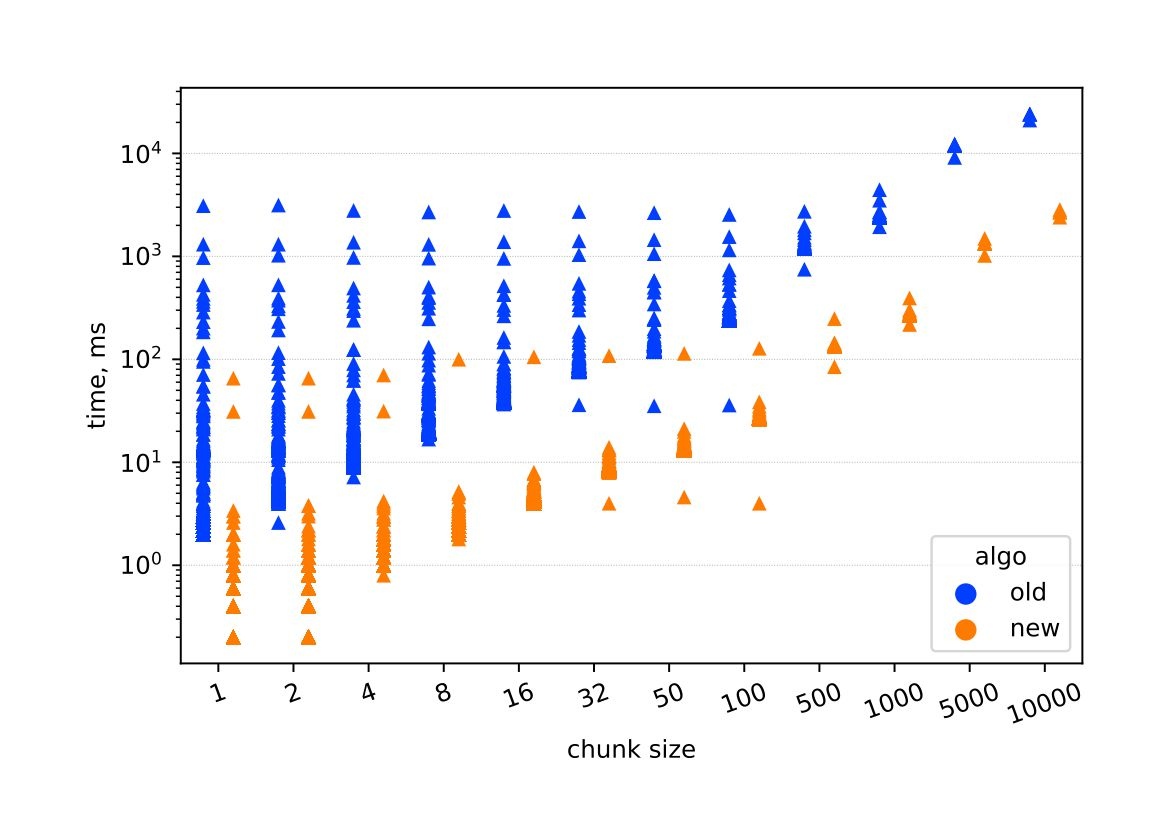
\includegraphics[width=\textwidth]{figures/st_old_new.pdf_1.jpg}  \caption{Query time}
    \label{fig:subim1}
    \end{subfigure}%
    % \hfill
    \begin{subfigure}[b]{0.5\textwidth}
    \centering
    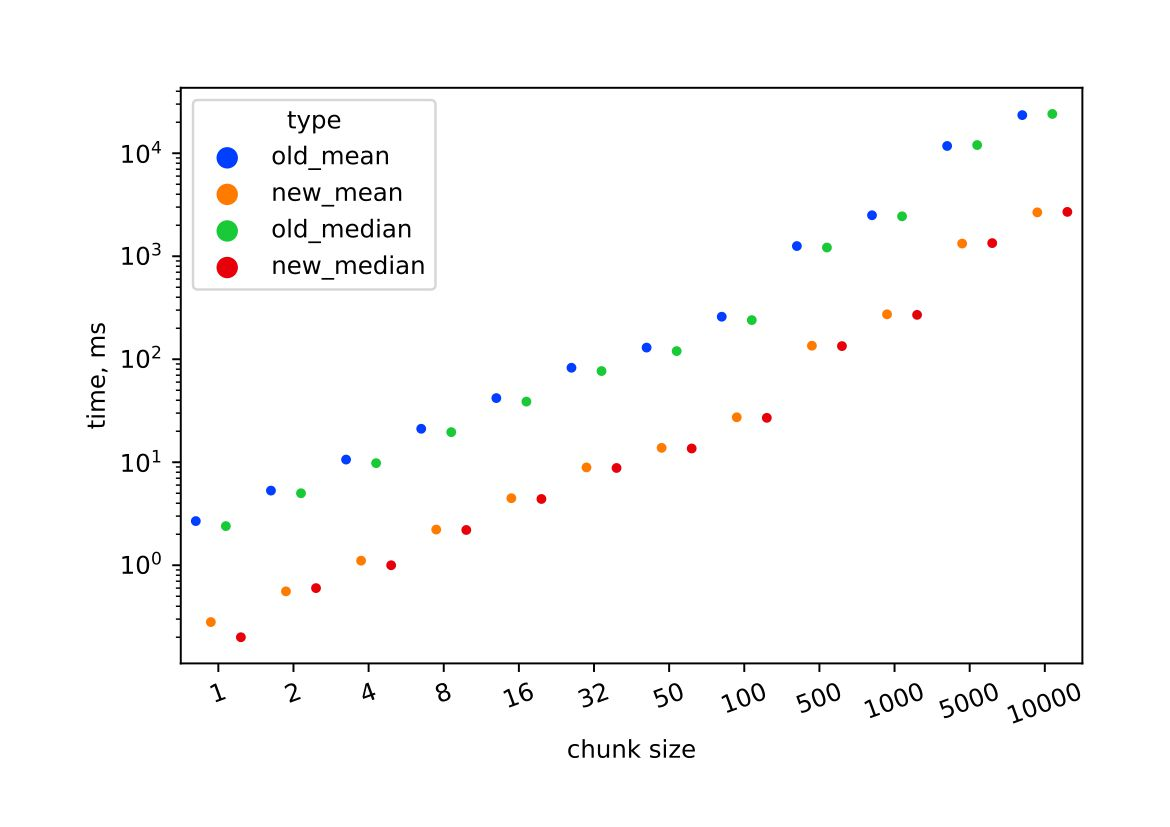
\includegraphics[width=\columnwidth]{figures/st_old_new_mean&median.pdf_1.jpg} \caption{Median and mean query time}
    \label{fig:subim2}
    \end{subfigure} \caption{Grammar $G_1$ and Enzyme}
    \label{old_new}
        % \end{figure} 
    % \begin{figure}[h!]
    \begin{subfigure}[b]{0.5\textwidth}
    \centering
    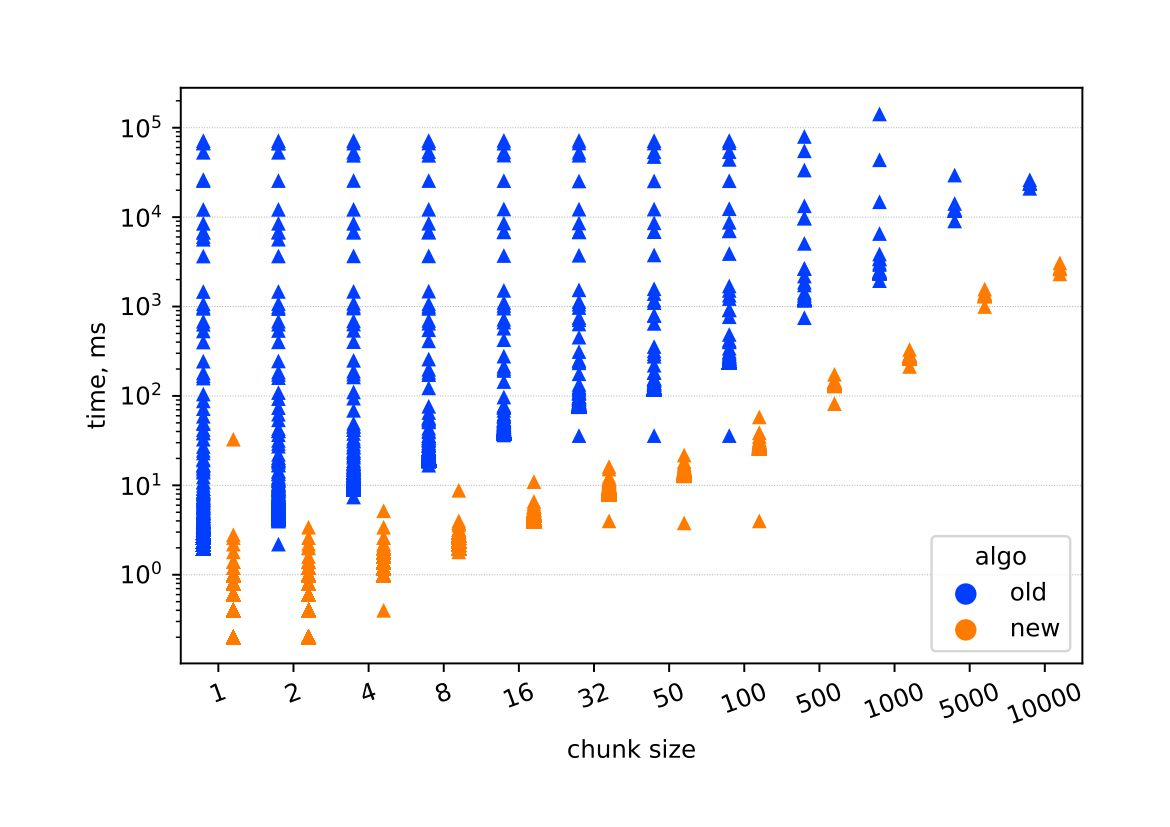
\includegraphics[width=\textwidth]{figures/subclass_old_new.pdf_1.jpg} \caption{Query time}
    \label{fig:subim1}
    \end{subfigure}%
    % \hfill
    \begin{subfigure}[b]{0.5\textwidth}
    \centering
    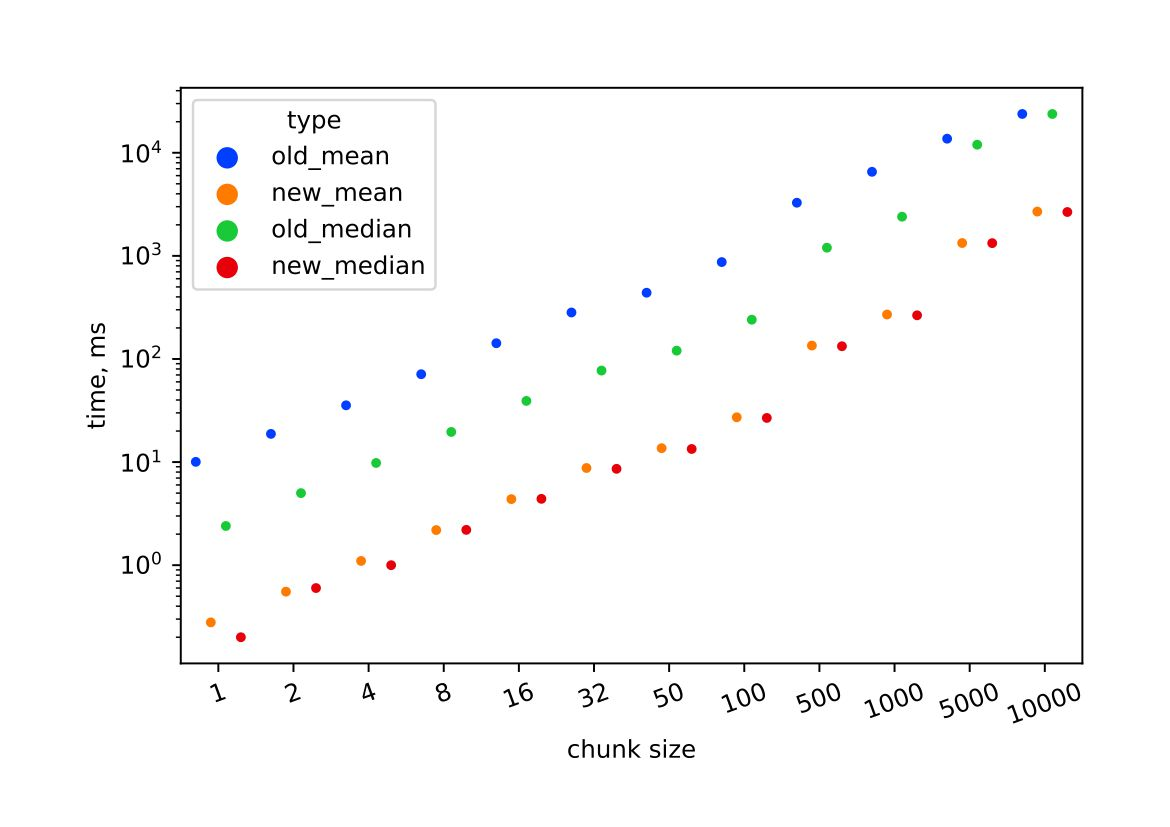
\includegraphics[width=\columnwidth]{figures/subclass_old_new_mean&median.pdf_1.jpg} \caption{Median and mean time}
    \label{fig:subim2}
    \end{subfigure} \caption{Grammar $G_2$ and Enzyme}
    \label{old_new2}
        \begin{subfigure}[b]{0.5\textwidth}
    \centering
    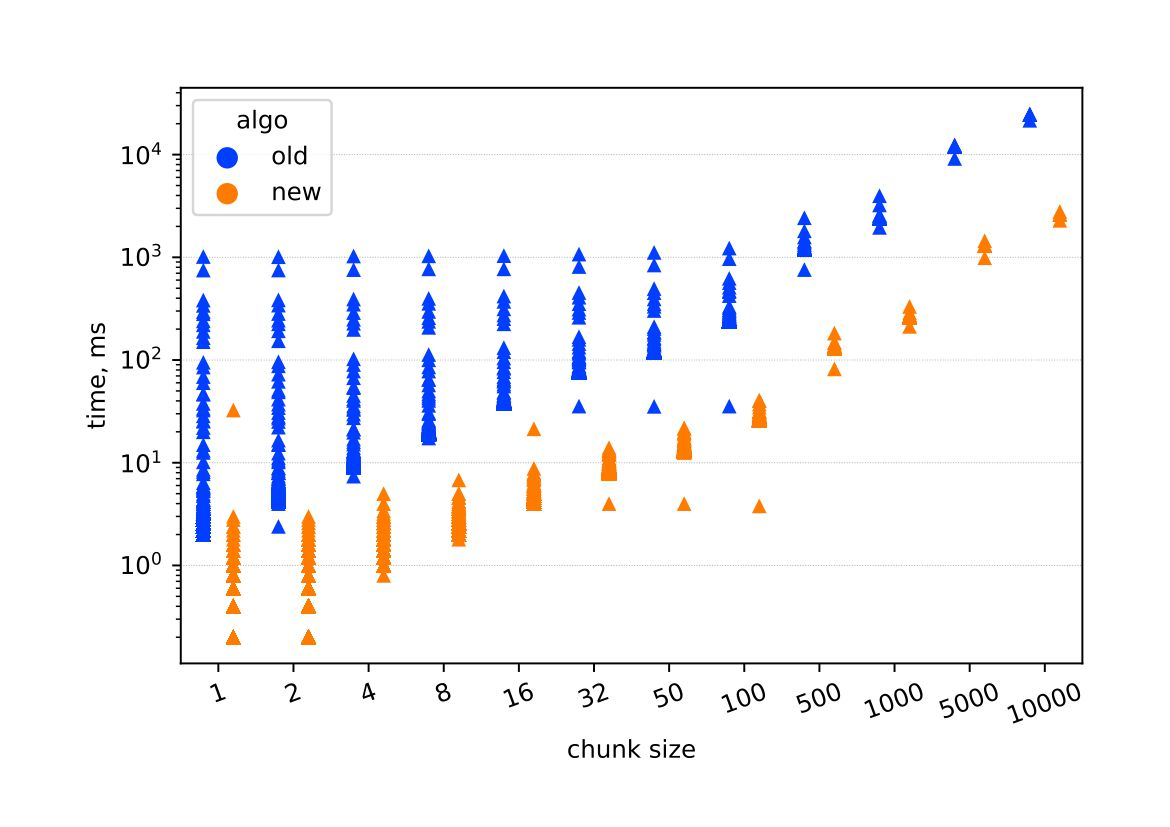
\includegraphics[width=\columnwidth]{figures/bt_old_new.pdf_1.jpg}  \caption{Query time}
    \label{fig:subim1}
    \end{subfigure}%
    % \hfill
    \begin{subfigure}[b]{0.5\textwidth}
    \centering
    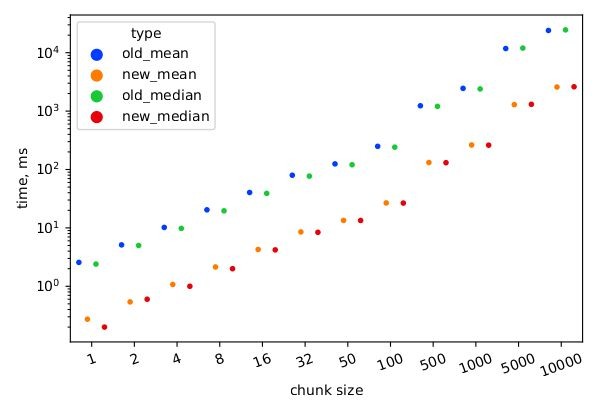
\includegraphics[width=\textwidth]{figures/bt_old_new_mean&median.pdf_1.jpg} \caption{Median and mean}
    \label{fig:subim2}
    \end{subfigure} \caption{Grammar $Geo$ and Enzyme}
\label{old_new3}
\end{figure}

    Similarly, the median and mean query time for each size of the set of start vertices are additionally allocated. These results show that the improved version of the algorithm not only spends an order of magnitude less time resources, but also is more stable on average on real-world graphs. This is especially noticeable in Fig.\ref{old_new2} which demonstrates the median and average time. For the modified algorithm these two indicators are almost equal.
    
The resulting solution was evaluated on the same hardware. Since, after the optimizations, the amount of consumed processor resources significantly decreased for both algorithms, it became possible to include the whole RDF graphs dataset for experimental study. The results of the all-pairs reachability queries evaluation are presented in tables~\ref{tab:all_pairs_rdf} -- \ref{tab:all_pairs_stat}. 

\begin{table*}[h!]
    \centering
    \begin{tabular}{| l | c | c | c | c |}
         \hline
         \multirow{Graph name} & \multicolumn{2}{c|}{$G_1$} & \multicolumn{2}{c|}{$G_2$}\\
         \cline{2-5}
         & time (sec) & \#answer & time (sec) & \#answer \\
         \hline
         \hline
         Core               & 0,02   & 204     & 0,01    & 214 \\
         Pathways           & 0,07   & 884     & 0,04    & 3117 \\
         Go hierarchy       & 3,68 & 588 976 & 5,4 & 738 937 \\
         Enzyme             & 0,22   & 396     & 0,17    & 8163 \\
         Eclass     & 1,5 & 90 994  & 0,98  & 96 163\\
         Geospecies         & 2,87   & 85      & 2,65    & 0 \\
         Go                 & 5,56  & 640 316 & 4,2   & 659 501 \\
         Taxonomy           & 45,47  & 151 706 & 36,07 & 2 112 637 \\
         \hline
    \end{tabular}
    \caption{Single thread all-pairs reachability performance results for RDFs: time in seconds, \textbf{\#answer} is a number of reachable pairs}
    \label{tab:all_pairs_rdf}
\end{table*}

\begin{table*}[h!]
    \centering
    \begin{tabular}{| l | c | c |}
         \hline
         \multirow{Graph name} &  \multicolumn{2}{c|}{$Geo$} \\
         \cline{2-3}
         & time (sec) & \#answer \\
         \hline
         \hline
         Enzyme & 5,7 & 14 267 542 \\
         Geospecies & 145,8 & 226 669 749 \\
         \hline
    \end{tabular}
    \caption{Single thread all-pairs reachability performance results for RDFs: time in seconds, \textbf{\#answer} is a number of reachable pairs}
    \label{tab:all_pairs_geo}
\end{table*}

\begin{table*}[h!]
    \centering
    \begin{tabular}{| l | c | c | c |}
         \hline
         \multirow{Graph name} &  \multicolumn{3}{c|}{$PointsTo$} \\
         \cline{2-4}
         & time (sec) & matrix time (sec) & \#answer \\
         \hline
         \hline
         Apache & -- & 536,7 & 92 806 768 \\
         Block  & 113,01 & 123,88 & 53 514 095  \\
         Fs     & 167,73  & 105,72 & 9 646 475\\
         Ipc    & 109,43 & 79,52 & 5 249 389 \\
         Lib    & 111,09 & 121,79 & 5 276 303 \\
         Mm     & 77,92 & 84,15 & 3 990 305  \\
         Net    & 160,64 & 206,29 & 8 833 403 \\
         Postgre  & -- & 969,88 & 90 661 446 \\
         Security & 115,75 & 181,7 & 5 593 387 \\
         Sound    & 120,14 & 133,64 & 6 085 269 \\
         Init     & 87,25 & 45,84 & 3 783 769 \\
         Arch     & 130,77 & 119,92  & 5 339 563 \\
         Crypto   & 128,8  & 122,09 & 5 428 237\\
         Drivers  & 371,18 & 279,39 & 18 825 025  \\
         Kernel   & 614,05 & 378,05 & 16 747 731 \\
         \hline
    \end{tabular}
    \caption{Single thread all-pairs reachability performance results: time in seconds, \textbf{\#answer} is a number of reachable pairs}
    \label{tab:all_pairs_stat}
\end{table*}



The results show that query evaluation time depends not only on a graph size or its sparsity, but also on an inner structure of the graph. For example, the relatively small graph Go hierarchy fully consists of edges used in queries $G_1$ and $G_2$, thus evaluation time for these queries is significantly bigger than for some bigger but more sparse graphs, for example, for Eclass graph. Note that the size of the answer is not a good metric, because, for example, answers for Geo query, and Enzyme and Geospecies graphs, are calculated faster than the answers for Go hierarchy. The creation of relevant metrics for CFPQ queries evaluation time prediction is a challenging problem by itself and should be tackled in the future.

The important results are demonstrated in Table~\ref{tab:all_pairs_geo}. Previous similar solution required more then 6900 seconds to evaluate the the Geo query for the Geospecies graph~\cite{10.1145/3335783.3335791}. Thus it shows that the performance of CFPQ for Neo4j was significantly improved.

% Results for graphs related to static code analysis are compared to Azimov's CFPQ algorithm based on matrix operations. The implementation from CFPQ\_PyAlgo repository\footnote{CFPQ\_PyAlgo repository: \url{https://github.com/JetBrains-Research/CFPQ_PyAlgo}, accessed: 05/05/2022} was taken as the implementation of the matrix CFPQ algorithm. This library contains the implementation for both scenarios, all pairs and single source. To perform matrix operations pygraphblas\footnote{pygraphblas repository: \url{https://github.com/Graphegon/pygraphblas}, accessed: 05/05/2022} is used. Pygraphblas is a python wrapper over the SuiteSparse library, which contains a set of sparse matrix algorithms to provide graph processing in terms of linear algebra.

The results for graphs related to static code analysis on all-pairs scenario are presented in Table~\ref{tab:all_pairs_stat}. The sign '--' in cells means that the respective query and graph require a considerable amount of memory during algorithm execution that leads to unpredictable time to get the result.
Although other queries related to code analysis can be evaluated in reasonable time even for relatively big graphs. Moreover, in some cases GLL-based CFPQ algorithm demonstrates comparable and even better time results than matrix based CFPQ algorithm. For example, Security graph is processed approximately one and a half times faster with GLL-based CFPQ algorithm than with matrix based CFPQ algorithm. Thus, CFPQ can be used to improve Neo4j-based code analysis systems. 

The another important scenario is the case when the start set is a single vertex. 
The results of the \texttt{single source reachablity} and \texttt{all paths reachability} queries related to RDF analysis are presented in figures~\ref{fig:ss-g1}--\ref{fig:ss-geo}.

\begin{figure}[h!]
    \centering
    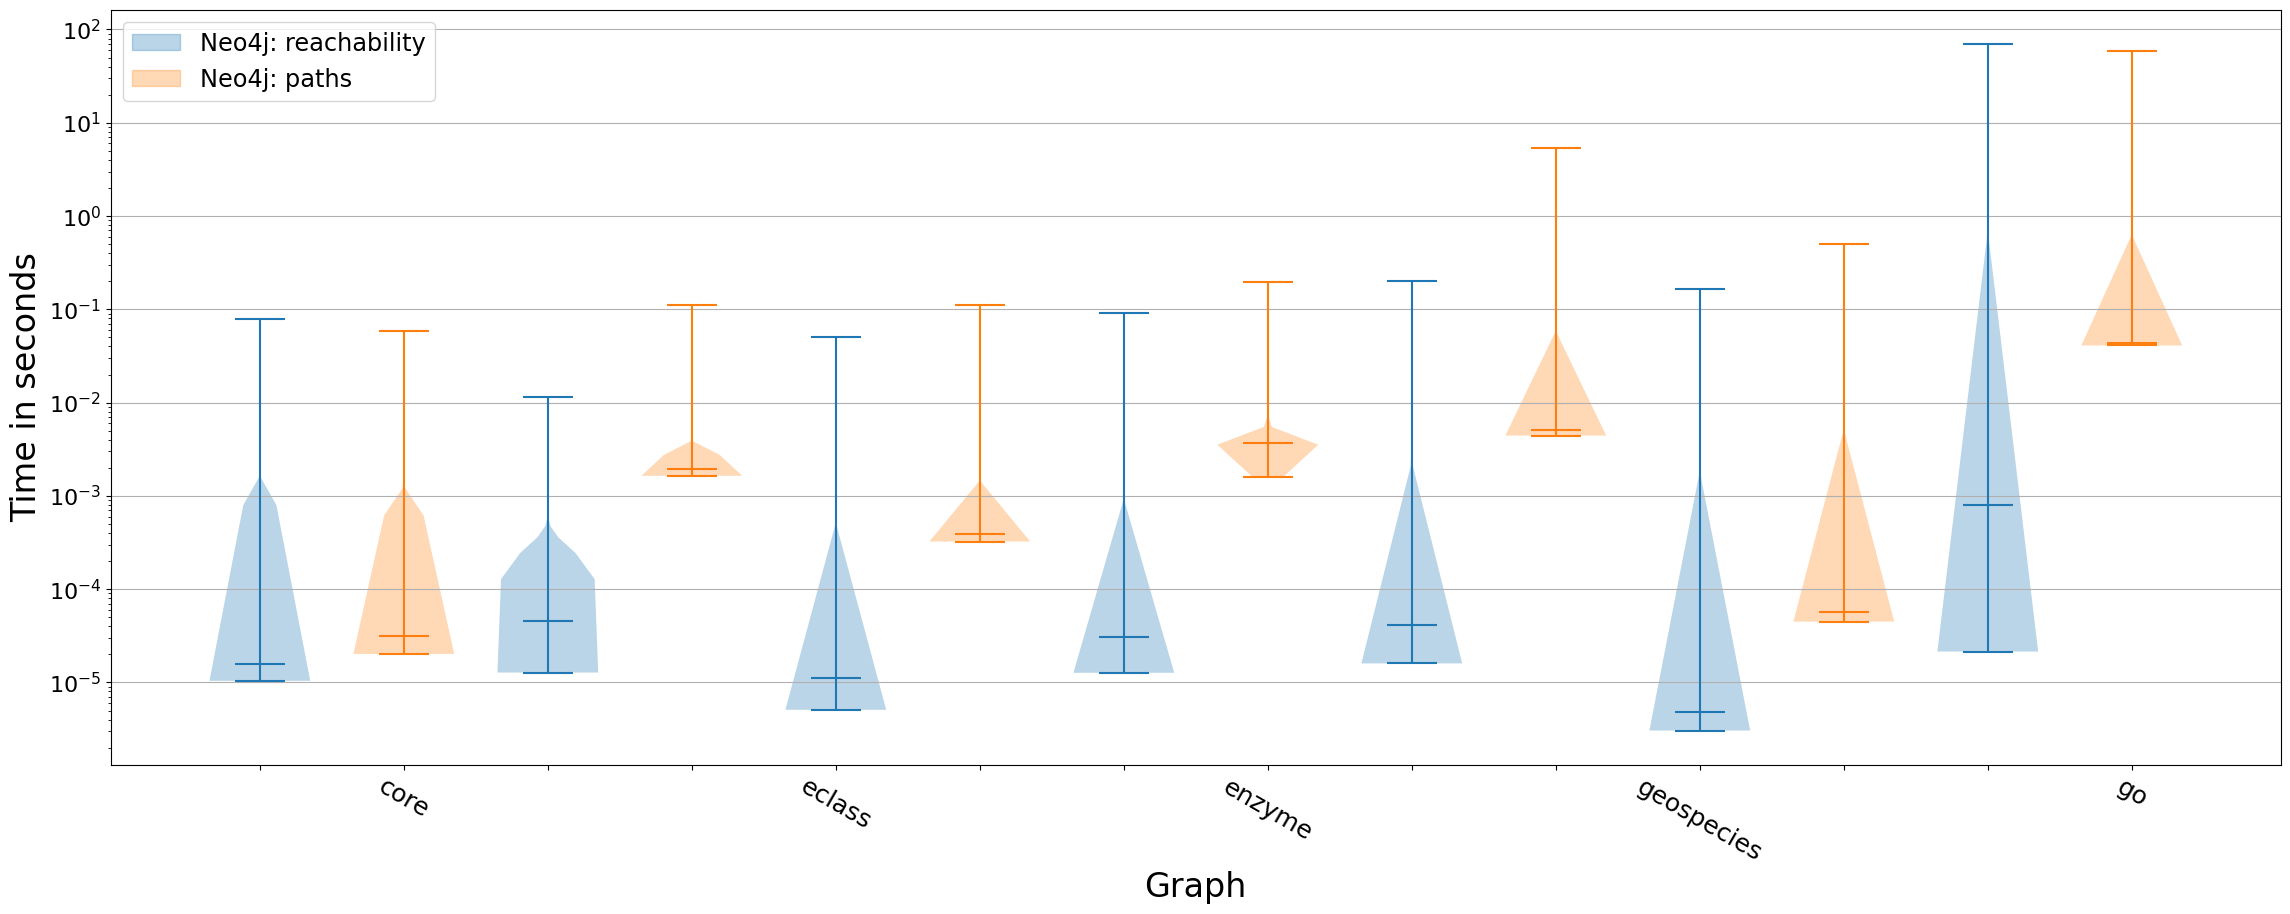
\includegraphics[width=\textwidth]{figures/ss-g1.png}
    \caption{Single source CFPQ results for queries related to RDF analysis and $G_1$}
    \label{fig:ss-g1}
\end{figure}

\begin{figure}[h!]
    \centering
    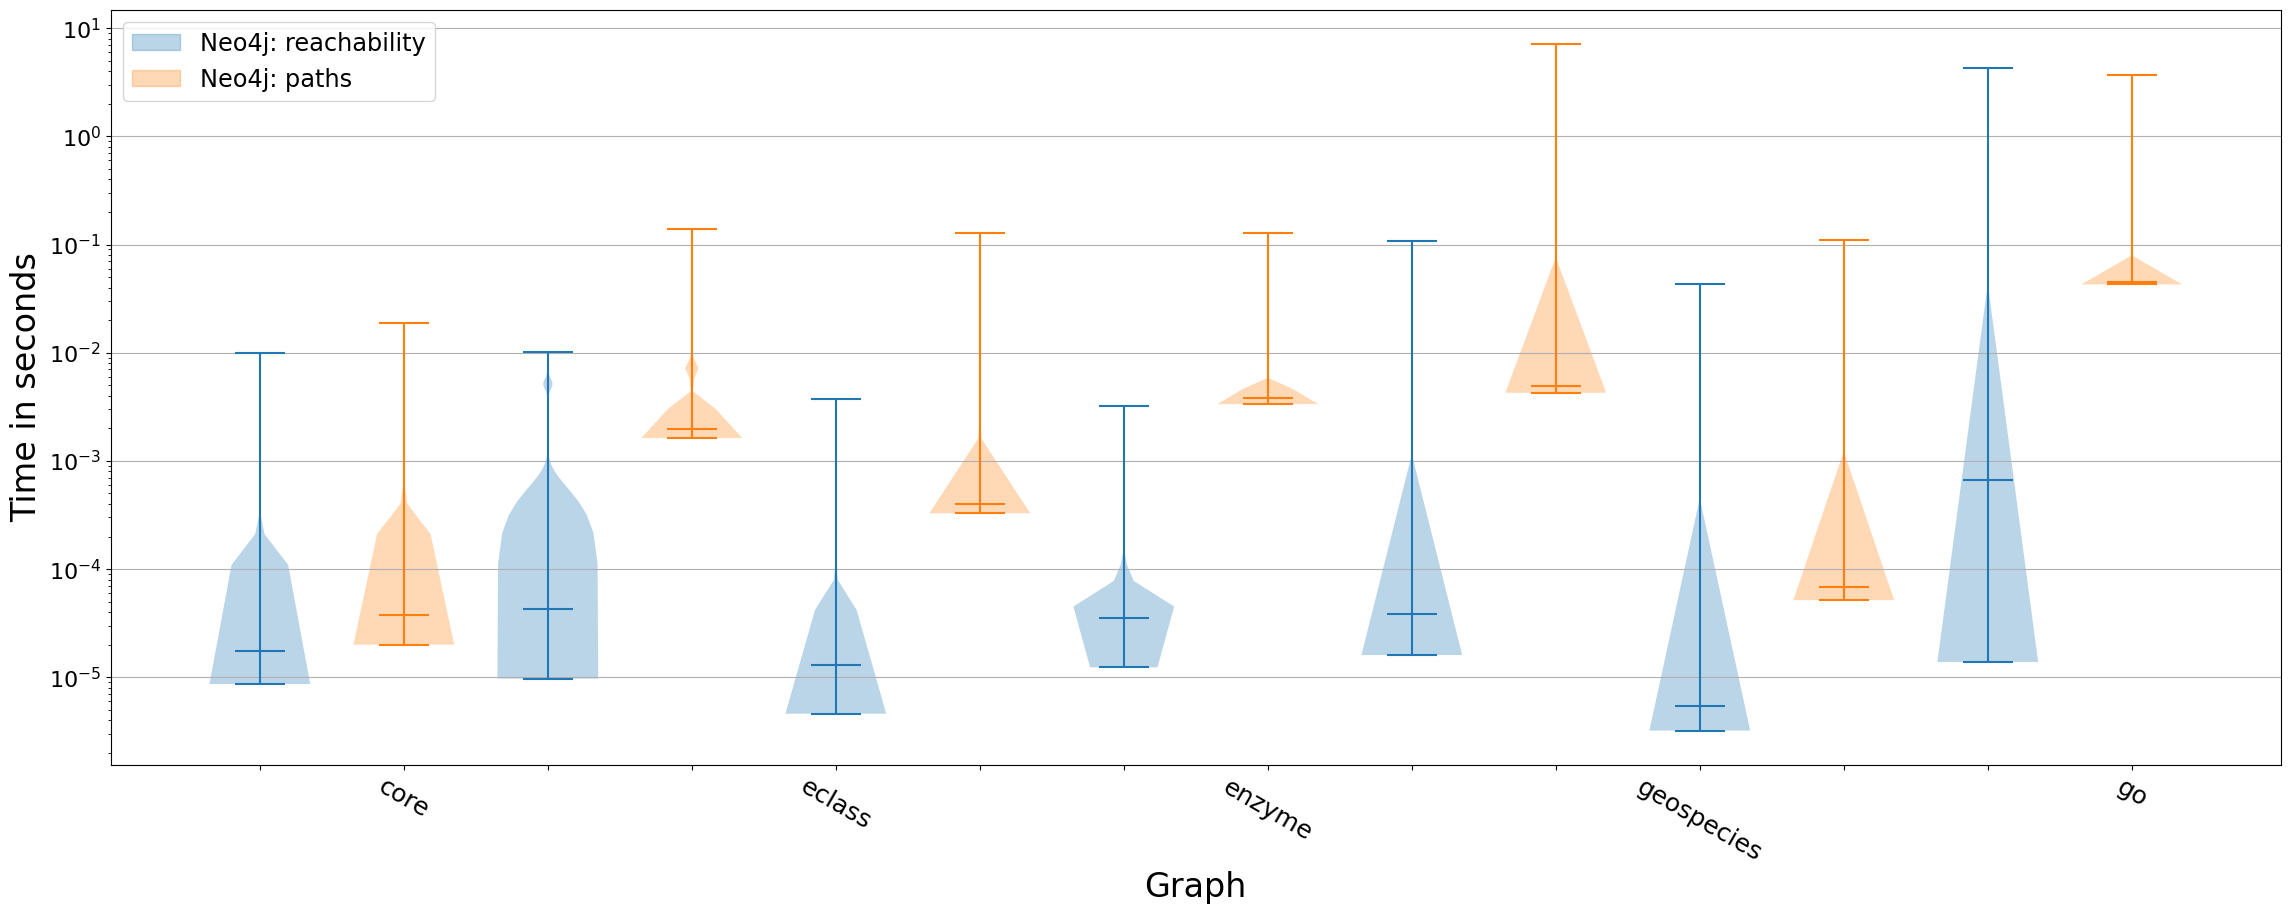
\includegraphics[width=\textwidth]{figures/ss-g2.png}
    \caption{Single source CFPQ results for queries related to RDF analysis and $G_2$}
    \label{fig:ss-g2}
\end{figure}

\begin{figure}[h!]
    \centering
    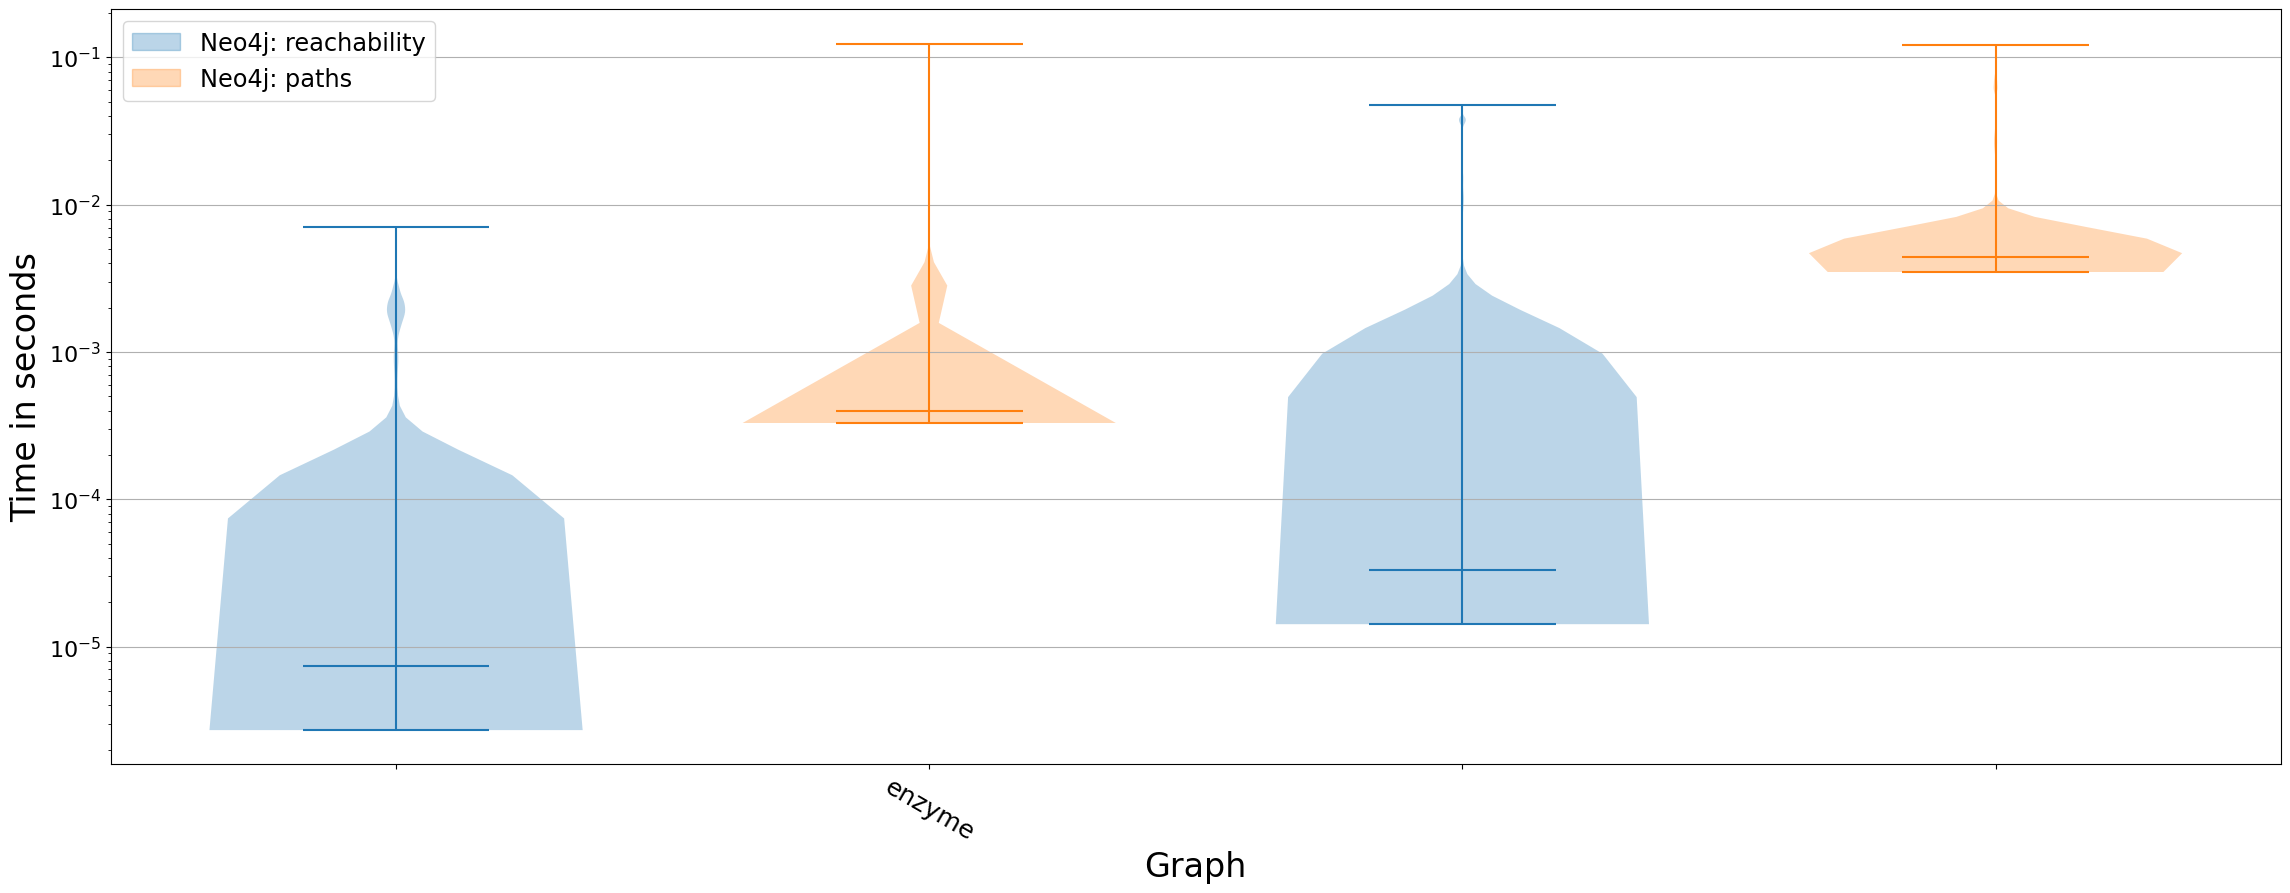
\includegraphics[width=\textwidth]{figures/ss-geo.png}
    \caption{Single source CFPQ results for queries related to RDF analysis and Geo}
    \label{fig:ss-geo}
\end{figure}

The go hierarchy graph is omitted because it fully connected with \textit{subClassOf} relation and GLL-based CFPQ algorithm does not handle well the SPPF construction for such specific case because of memory limits.

Firstly, it should be noted that the single-source queries are reasonably fast in both the \texttt{reachability} and the \texttt{all paths} cases: median time is less than $10^{-4}$ seconds for reachability queries, and is less than $10^{-1}$ seconds for \texttt{all paths} queries. Even for queries $G_1$ and $G_2$, which return relatively small answers, time required for the all paths queries is bigger than for reachability queries. Also there are some "heavy" cases when both scenarios require relatively a big amount of time to get the result. Moreover, for such cases the time for \texttt{reachability} and \texttt{all-paths} is comparable in contradiction to others. It should be due to the fact that often in single source scenario the memory allocation for SPPF construction require relatively significant amount of time. Thus, there is a noticeable difference between \texttt{reachability} and \texttt{all-paths} scenarios.

The results of the \texttt{single source reachablity} and \texttt{all paths} queries  related to static code analysis are presented in figure~\ref{fig:ss-stat}. Here is also the comparison with matrix based CFPQ algorithm. 
This is perhaps the most significant result, which shows that as a result of the optimizations, both the  for paths and the calculation of the fact of reachability are orders of magnitude faster than the execution of the same queries using the matrix algorithm.

\begin{figure}
    \centering
    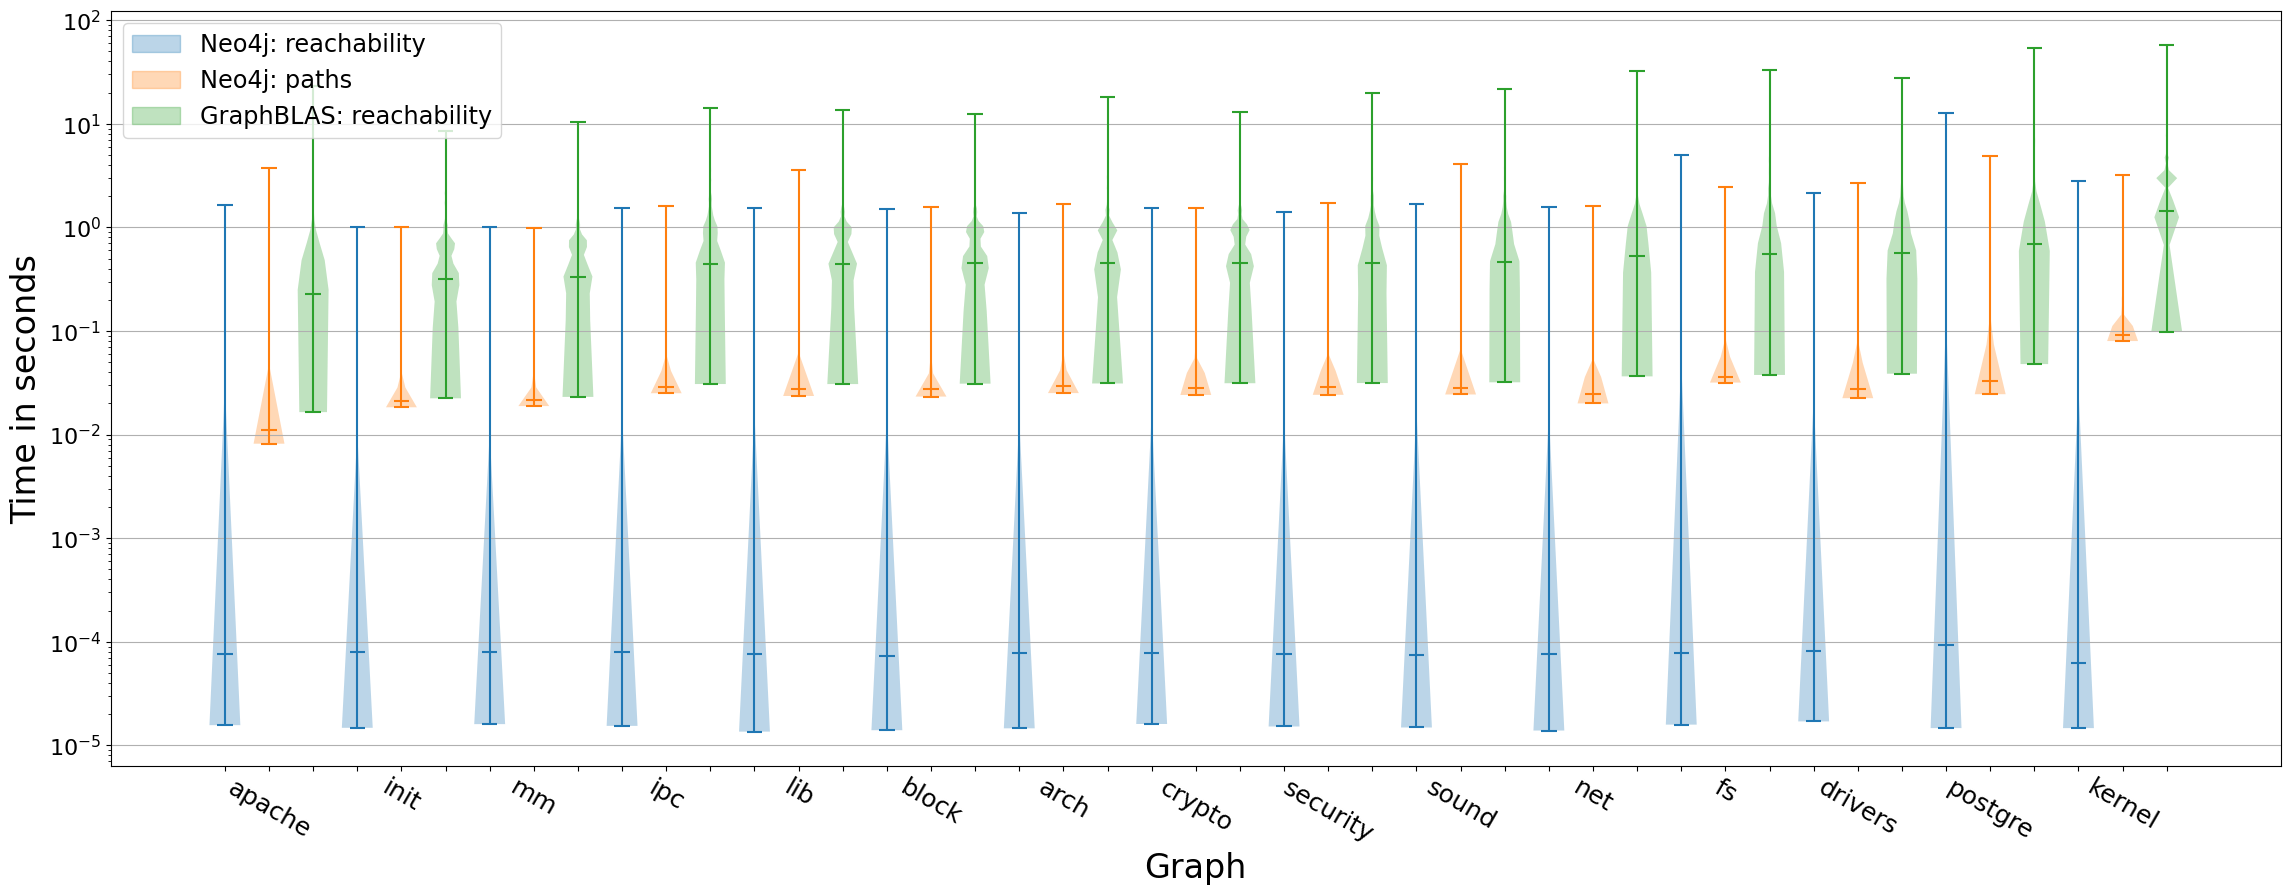
\includegraphics[width=\textwidth]{figures/stat-m.png}
    \caption{Single source CFPQ results for queries related to static code analysis}
    \label{fig:ss-stat}
\end{figure}

It is noticeable that the execution results are similar to results of the previous experiment. The execution time for all graphs except Postgre graph is less than $10^2$ seconds. Moreover, median time is less than $10^{-4}$ seconds for all processing sets.

To conclude, the analysis of the obtained results showed that the modified GLL algorithm can be effectively used on real-world graphs to solve the both problems: reachability and all-paths context-free path querying problems.
The obtained results make relevant further research aimed at both improving this algorithm and implementation, and its full integration into the Neo4j graph database.